\documentclass{beamer}
\usepackage{relsize}
\usepackage{color}

\usepackage{listings}
\usetheme{CambridgeUS}
%\usepackage{beamerthemesplit} % new 
\usepackage{enumitem}
\usepackage{amsmath}                    % See geometry.pdf to learn the layout options. 
\usepackage{amsthm}                   % See geometry.pdf to learn the layout options. There 
\usepackage{amssymb}                    % See geometry.pdf to learn the layout options. 
\usepackage[utf8]{inputenc} 
\usepackage{graphicx}
\usepackage[english,bulgarian]{babel}

\lstset{language=C++,
                basicstyle=\ttfamily,
                keywordstyle=\color{blue}\ttfamily,
                stringstyle=\color{red}\ttfamily,
                commentstyle=\color{green}\ttfamily,
                morecomment=[l][\color{magenta}]{\#}
}

\newtheorem{mydef}{Дефиниция}[section]
\newtheorem{lem}{Лема}[section]
\newtheorem{thm}{Твърдение}[section]

\DeclareMathOperator{\restrict}{\upharpoonright}

\setitemize{label=\usebeamerfont*{itemize item}%
  \usebeamercolor[fg]{itemize item}
  \usebeamertemplate{itemize item}}

\setbeamercovered{transparent}



\begin{document}
\title[Структури от данни и програмиране]{Работа с графи} 
\author{Калин Георгиев} 
\frame{\titlepage} 

\section{Интуиция} 


\begin{frame}
\centerline{Интуиция}
\end{frame}


\begin{frame}[fragile]
\frametitle{Възли, дъги, цени}

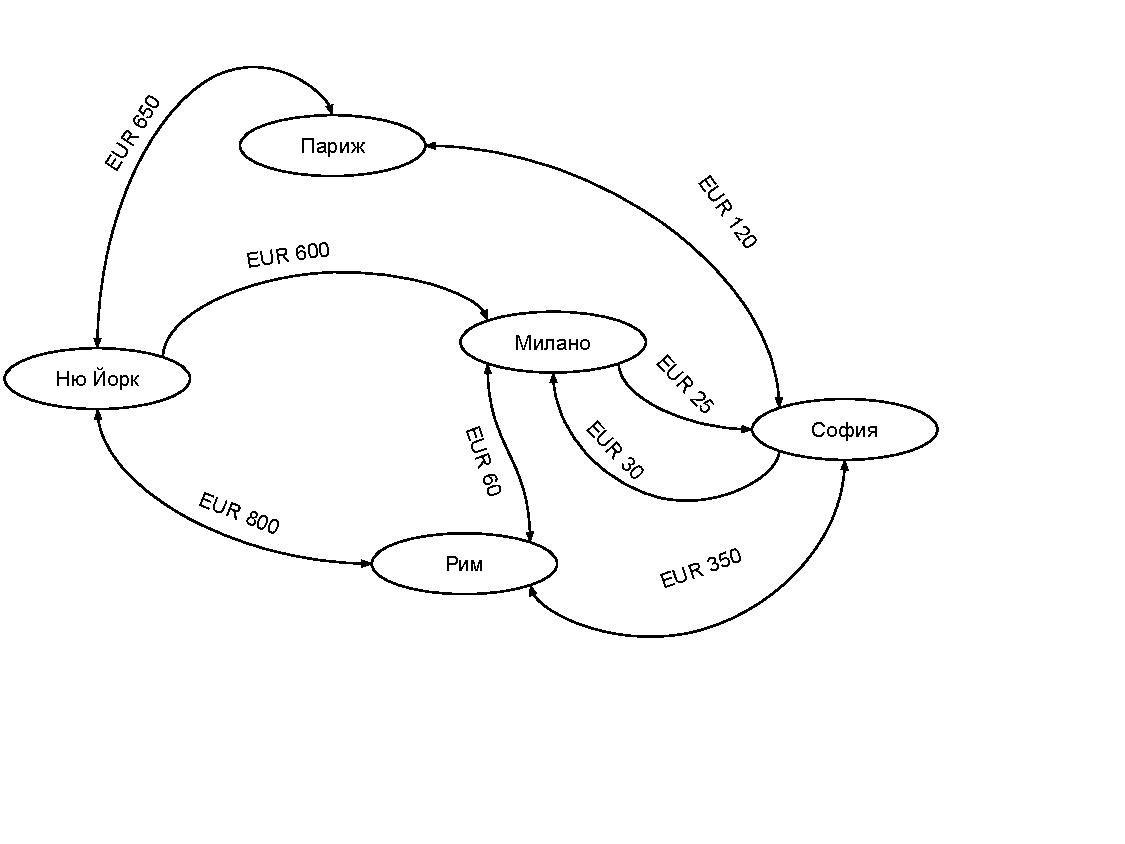
\includegraphics[width=13cm]{images/graph_cities}

\end{frame}


\begin{frame}[fragile]
\frametitle{Възли, дъги, цени}

\begin{center}
  $G=<V,E,w>$, $E=V \times V$, $w:E \rightarrow R$
\end{center}

\begin{columns}[t]
  \begin{column}{0.55\textwidth}
    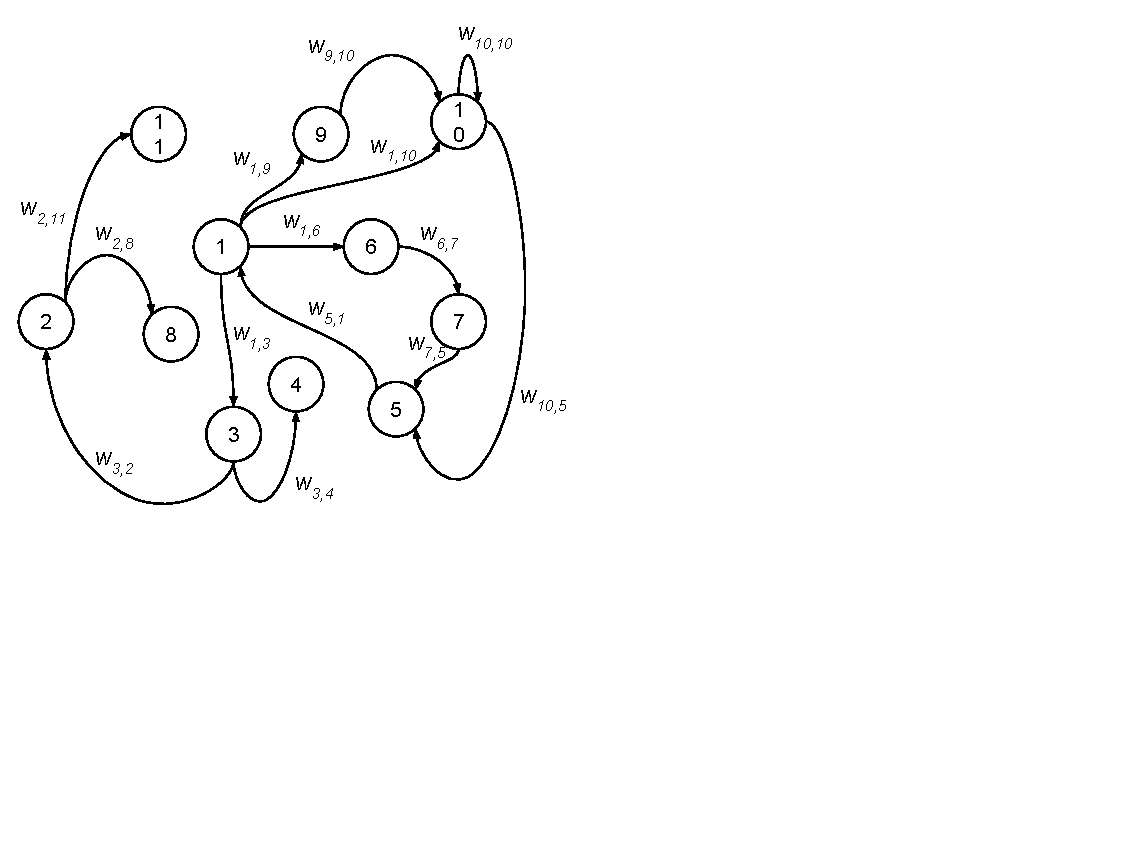
\includegraphics[width=13cm]{images/graph_numbers_weight}
  \end{column}
  \begin{column}{0.45\textwidth}
    \begin{flushleft}

    \vspace{-250px}
      Матрица с тегла
      $W_{|V|\times|V|}:(w)_{u,v}=w(u,v)$
      
    \end{flushleft}
  \end{column}
\end{columns}



\end{frame}



\begin{frame}[fragile]
\frametitle{Възли, дъги, без цени}

\begin{center}
  $G=<V,E>$, $E=V \times V$
\end{center}

\begin{columns}[t]
  \begin{column}{0.55\textwidth}
    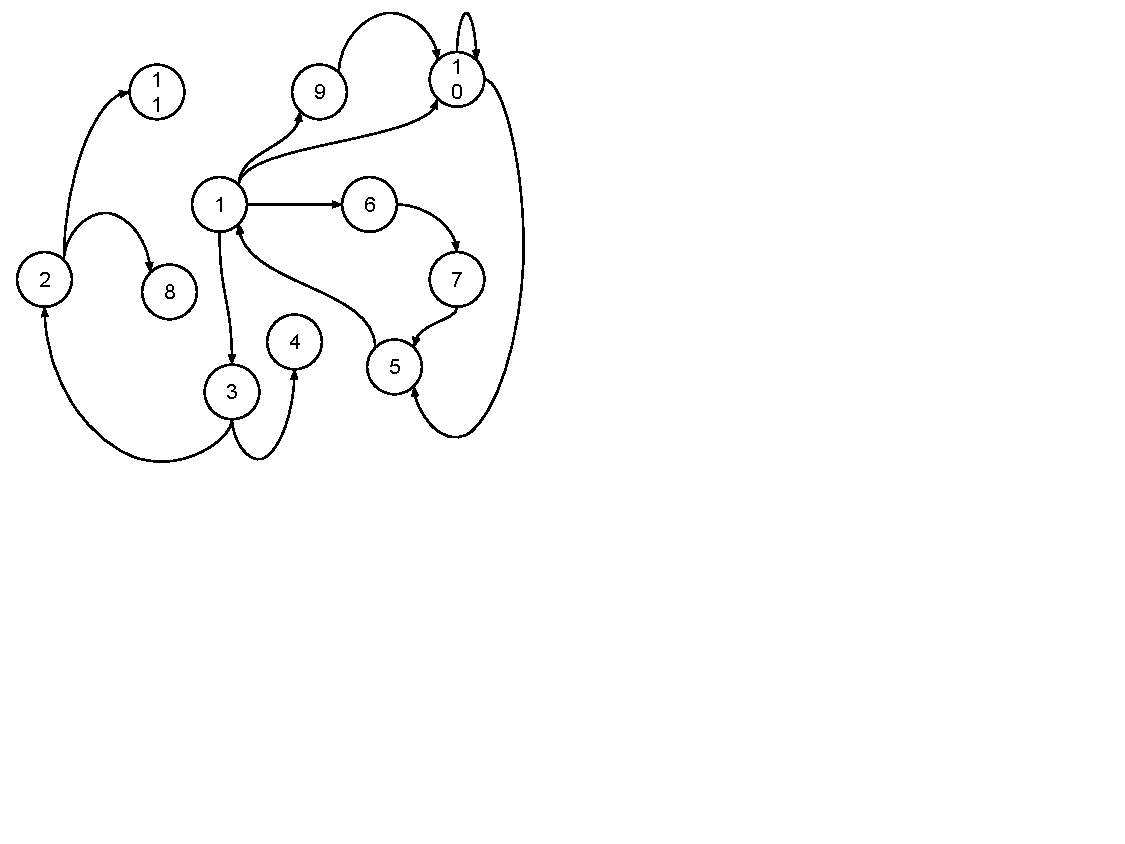
\includegraphics[width=13cm]{images/graph_numbers}
  \end{column}
  \begin{column}{0.45\textwidth}
    \begin{flushleft}

    \vspace{-250px}
      Матрица на съседство

      Incidence Matrix

      $A_{|V|\times|V|}:(a)_{u,v} \in \{true,false\}$

      $(a)_{u,v} \leftrightarrow(u,v)\in E$
      
    \end{flushleft}
  \end{column}
\end{columns}



\end{frame}



\begin{frame}[fragile]
\frametitle{Представяне}

\begin{itemize}
  \item Матрица
  \item Списък със съседи 
\end{itemize}

\end{frame}


\begin{frame}
\centerline{Прости операции. Сериализация}
\end{frame}

\begin{frame}
\centerline{Обхождания и търсене на път}
\end{frame}

\begin{frame}[fragile]
\frametitle{Обхождане в дълбочина с рекурсия и стек}
 

 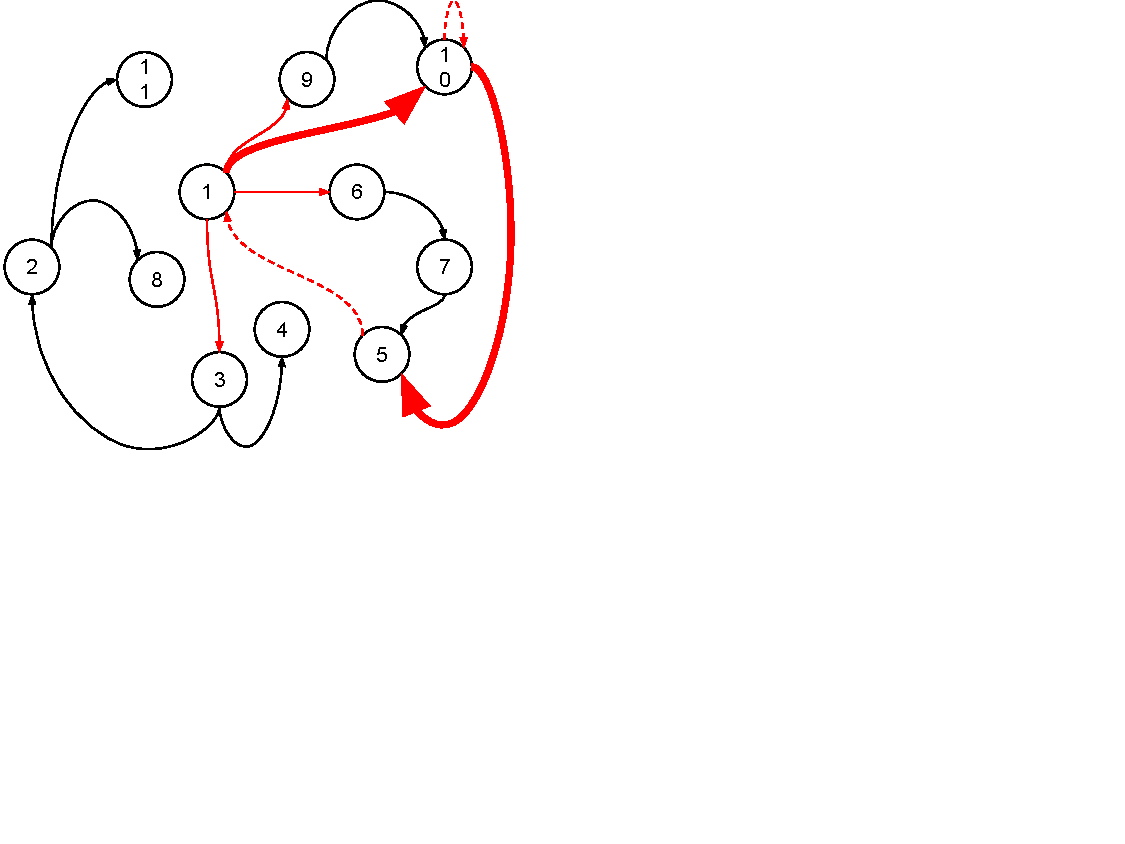
\includegraphics[width=13cm]{images/graph_dfs}


\end{frame}

\begin{frame}[fragile]
\frametitle{Обхождане в дълбочина}
 

\begin{columns}[t]
  \begin{column}{0.55\textwidth}
    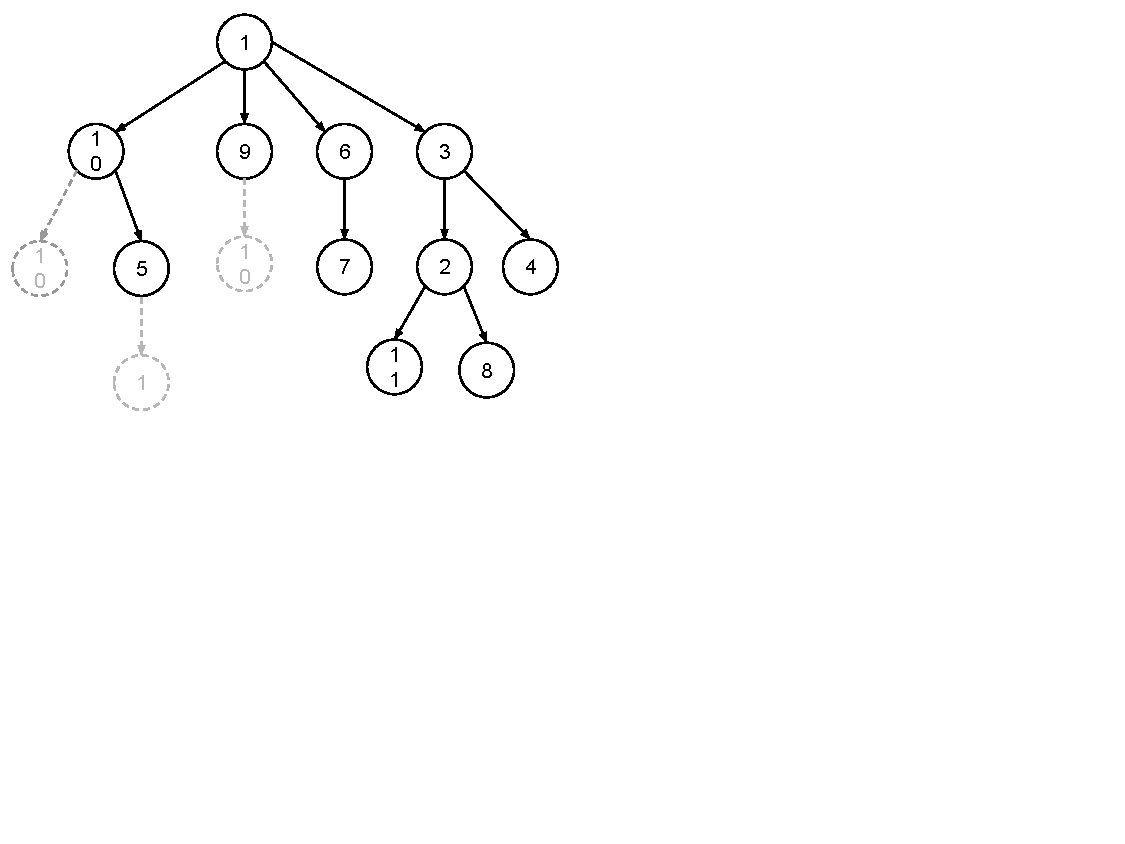
\includegraphics[width=12cm]{images/graph_span}
  \end{column}
  \begin{column}{0.45\textwidth}
  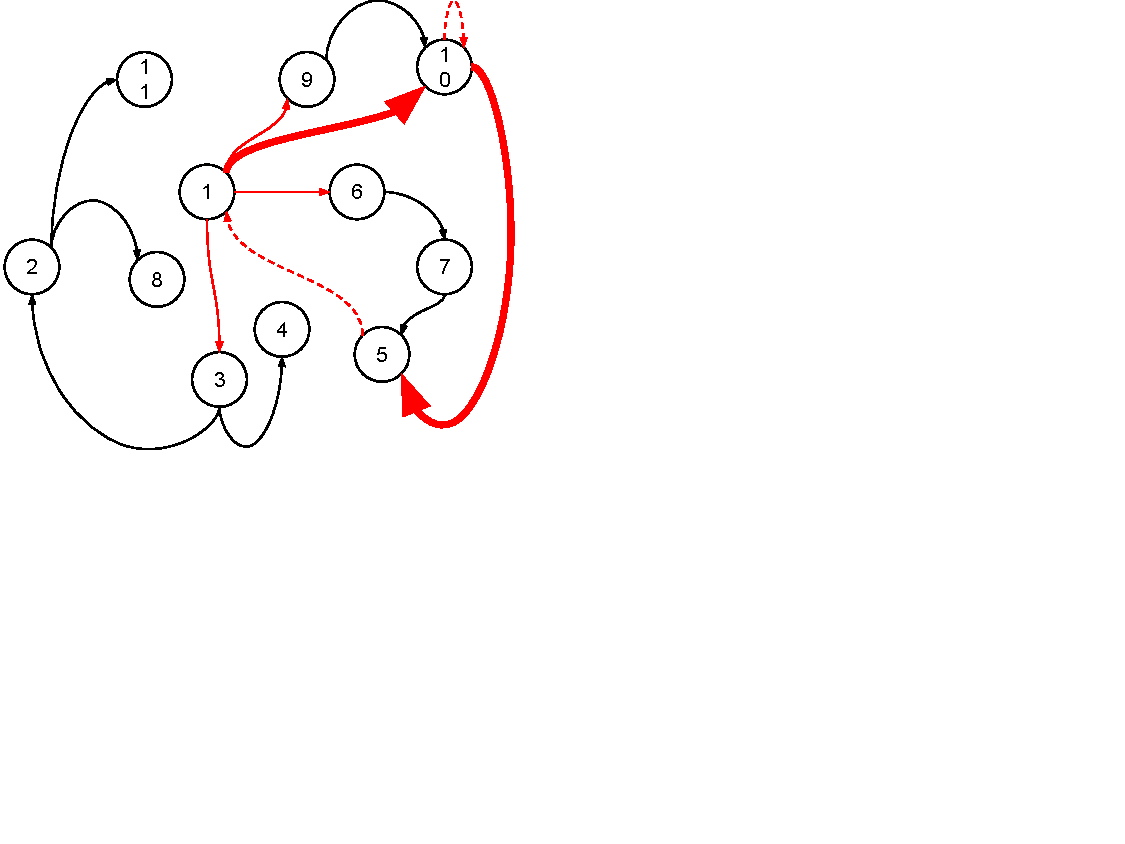
\includegraphics[width=10cm]{images/graph_dfs}
  \end{column}
\end{columns}

 


\end{frame}


\begin{frame}[fragile]
\frametitle{Обхождане в дълбочина}
 
\begin{columns}[t]
  \begin{column}{0.55\textwidth}
    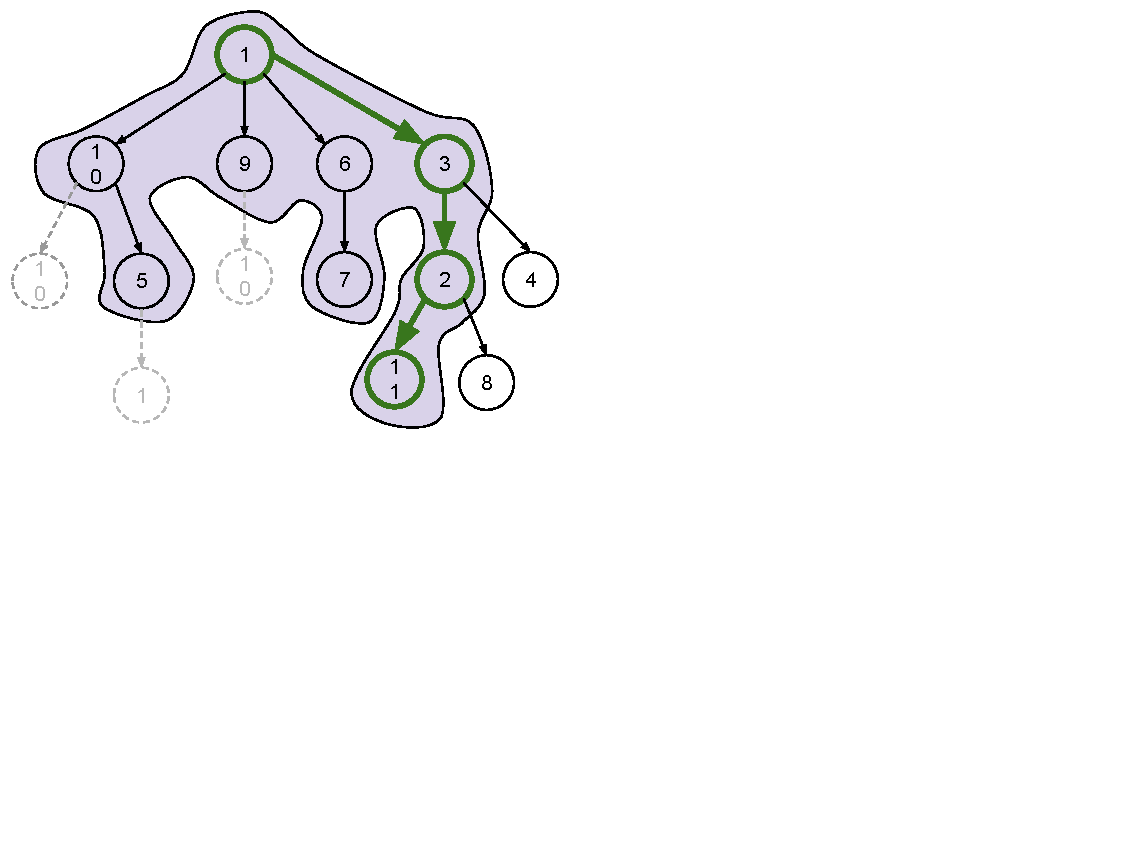
\includegraphics[width=12cm]{images/graph_dfs_2}
  \end{column}
  \begin{column}{0.45\textwidth}
  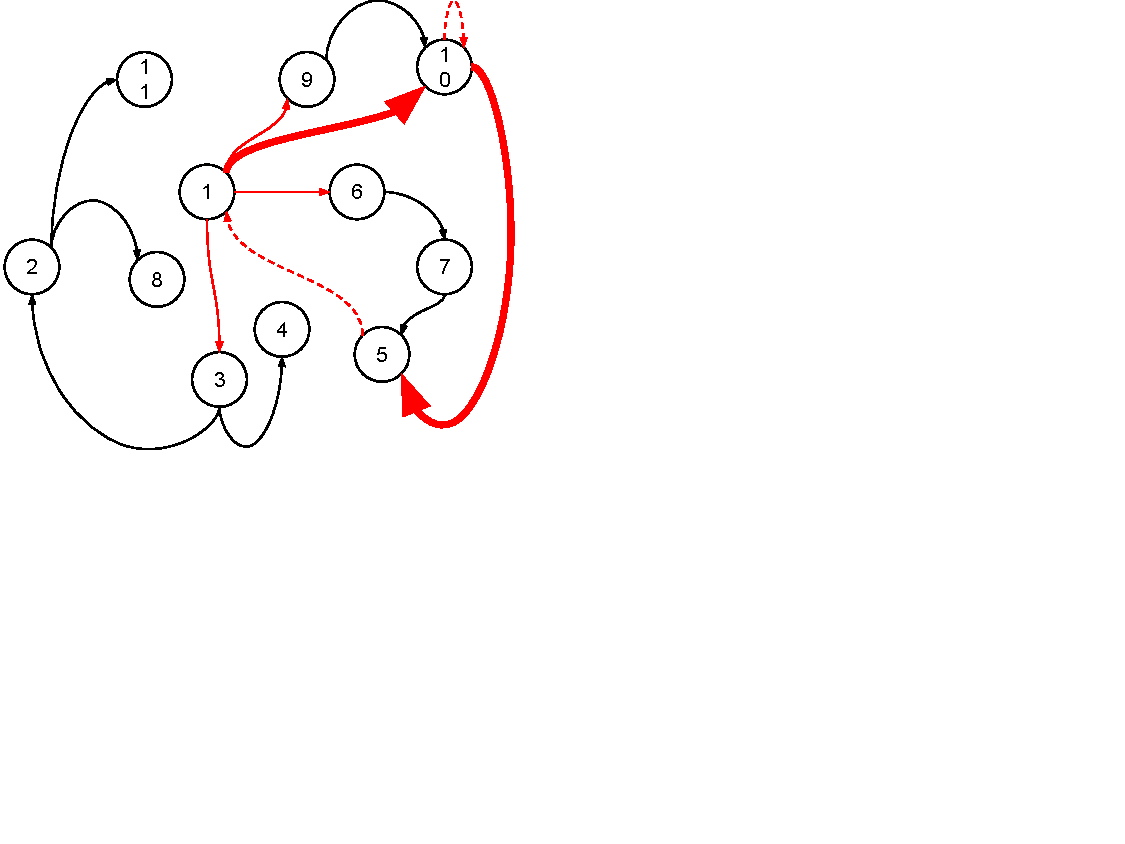
\includegraphics[width=10cm]{images/graph_dfs}
  \end{column}
\end{columns}

 

\end{frame}

\begin{frame}[fragile]
\frametitle{Обхождане в широчина}
 

\begin{columns}[t]
  \begin{column}{0.65\textwidth}
 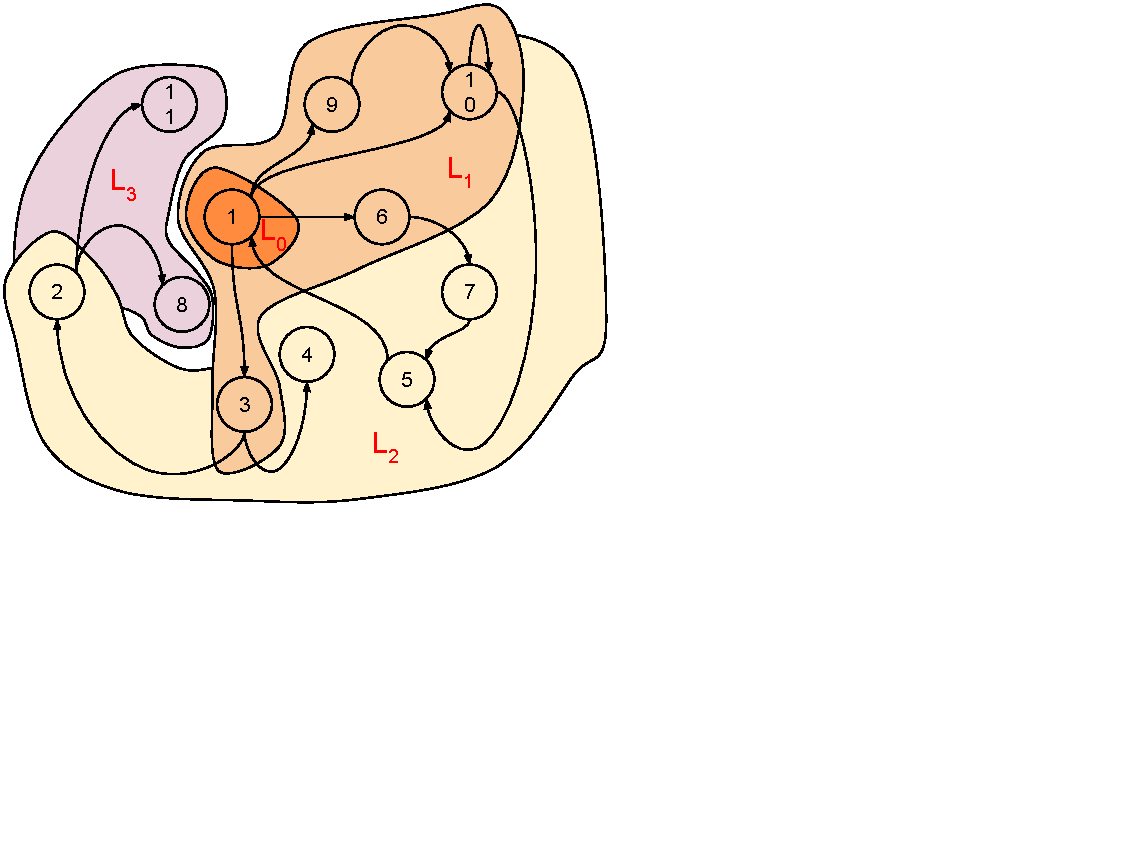
\includegraphics[width=13cm]{images/graph_levels}
 \end{column}
  \begin{column}{0.35\textwidth}
  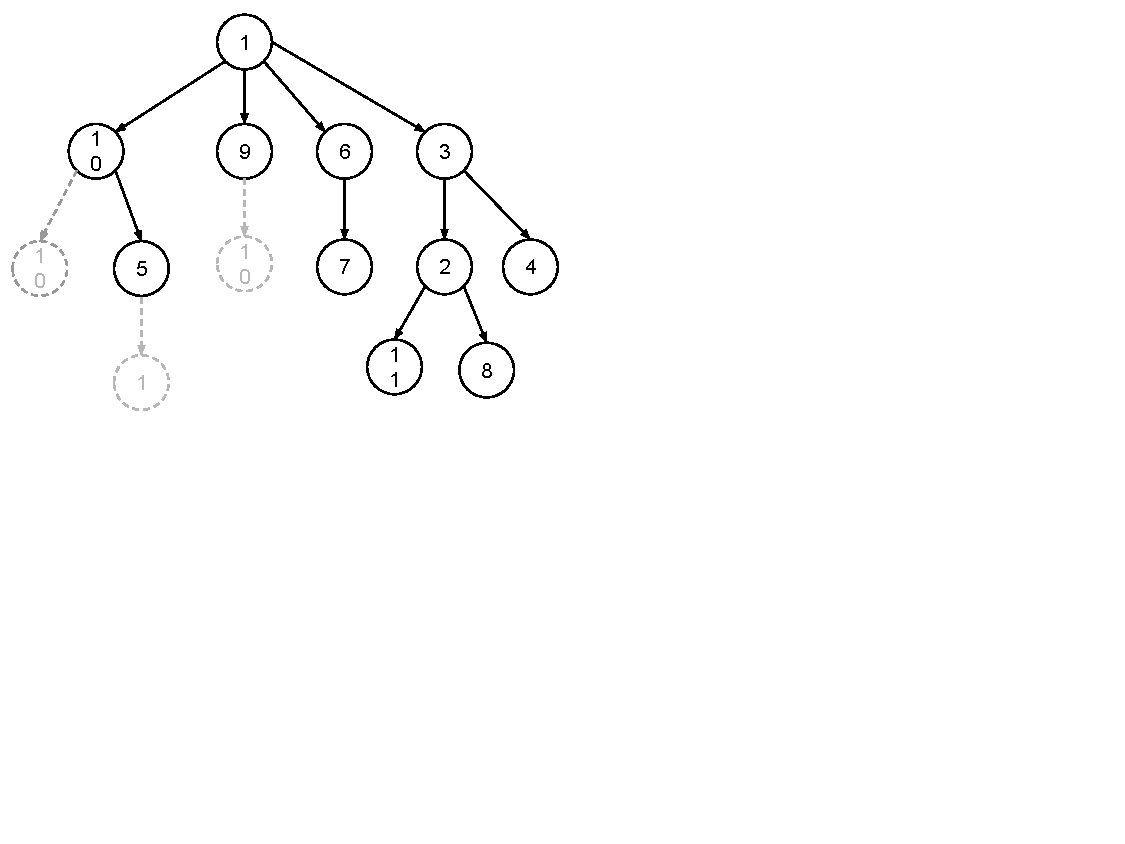
\includegraphics[width=9cm]{images/graph_span}
  \end{column}
\end{columns}

 

\end{frame}


\begin{frame}
\centerline{Въпроси?}
\end{frame}


\end{document}

\begin{columns}[t]
  \begin{column}{0.55\textwidth}

  \end{column}
  \begin{column}{0.45\textwidth}

  \end{column}
\end{columns}


